% fig_2_1_three_deficiencies.tex
% Three-panel diagram showing deficiencies in existing augmentation approaches
% Compile: pdflatex fig_2_1_three_deficiencies.tex
\documentclass[tikz,border=5pt]{standalone}

\usepackage[T1]{fontenc}
\usepackage[utf8]{inputenc}
\usepackage{amsmath,amssymb}
\usepackage{tikz}
\usetikzlibrary{arrows.meta, positioning, shapes.geometric, calc, patterns, decorations.markings}

% ── Color palette ──────────────────────────────────────────────────
\definecolor{classBlue}{HTML}{1565C0}
\definecolor{classOrange}{HTML}{EF6C00}
\definecolor{syntheticGreen}{HTML}{2E7D32}
\definecolor{warningRed}{HTML}{D32F2F}
\definecolor{checkGreen}{HTML}{4CAF50}
\definecolor{panelBg}{HTML}{FAFAFA}
\definecolor{arrowGray}{HTML}{455A64}
\definecolor{questionGray}{HTML}{757575}
\definecolor{barBlue}{HTML}{90CAF9}
\definecolor{datasetIcon}{HTML}{5C6BC0}

\begin{document}
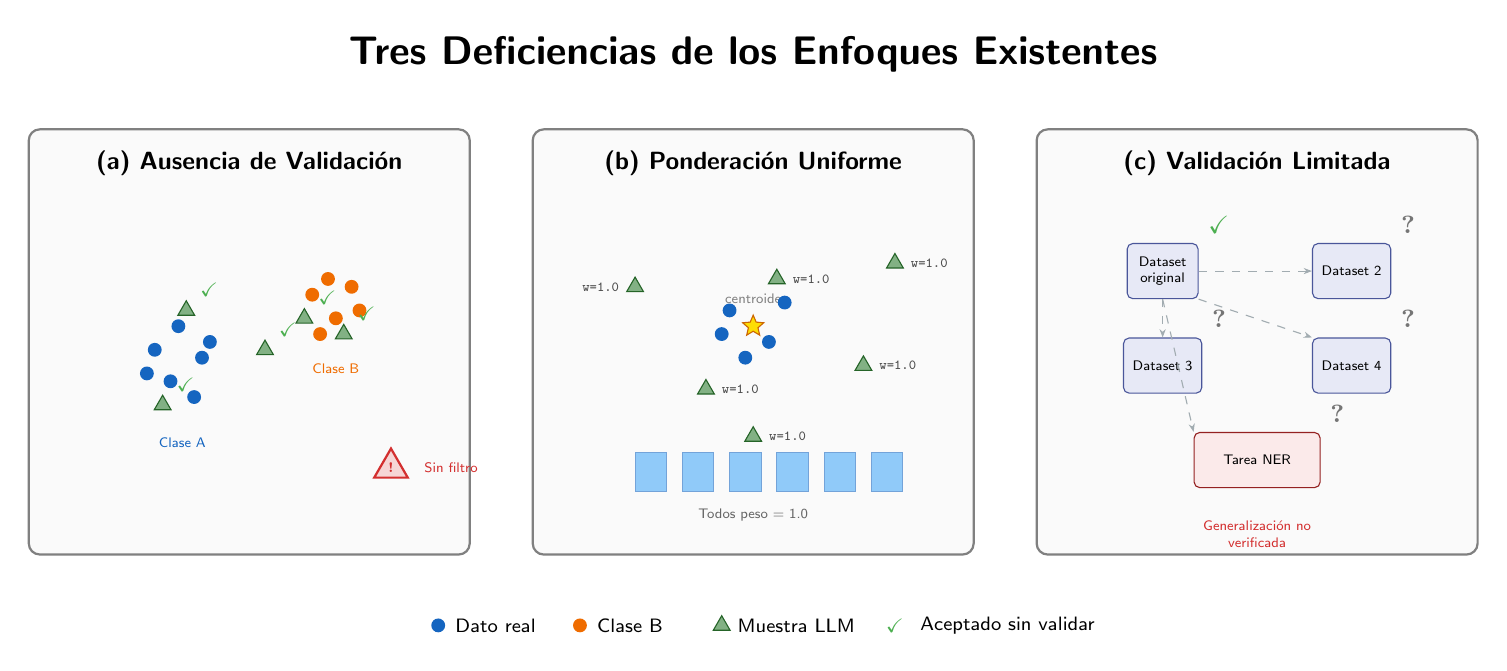
\begin{tikzpicture}[
    % ── shared styles ───────────────────────────────────────────────
    panel/.style={
        draw=black!50, thick, rounded corners=4pt, fill=panelBg,
    },
    panel title/.style={
        font=\sffamily\bfseries\small, anchor=north,
    },
    panel label/.style={
        font=\sffamily\scriptsize\itshape, text=black!60, anchor=north,
    },
    real blue/.style={circle, fill=classBlue, inner sep=0pt, minimum size=5pt},
    real orange/.style={circle, fill=classOrange, inner sep=0pt, minimum size=5pt},
    synth tri/.style={
        regular polygon, regular polygon sides=3,
        fill=syntheticGreen!60, draw=syntheticGreen!80!black,
        inner sep=0pt, minimum size=7pt,
    },
    checkmark/.style={font=\scriptsize\bfseries, text=checkGreen},
    weight label/.style={font=\tiny\ttfamily, text=black!70},
    dataset box/.style={
        rectangle, rounded corners=2pt, draw=datasetIcon!80!black,
        fill=datasetIcon!15, minimum width=0.9cm, minimum height=0.7cm,
        font=\sffamily\tiny, align=center,
    },
]

% =============================================================
%  Layout constants
% =============================================================
\def\pw{5.6}   % panel width
\def\ph{5.4}   % panel height
\def\gx{6.4}   % horizontal gap center-to-center

% =============================================================
%  Main title
% =============================================================
\node[font=\sffamily\Large\bfseries, anchor=south] at (1*\gx, 0.5*\ph+0.6)
    {Tres Deficiencias de los Enfoques Existentes};

% =============================================================
%  PANEL (a) -- Ausencia de Validacion
% =============================================================
\begin{scope}[shift={(0,0)}]
  \draw[panel] (-0.5*\pw,-0.5*\ph) rectangle (0.5*\pw,0.5*\ph);
  \node[panel title] at (0, 0.5*\ph-0.15) {(a) Ausencia de Validaci\'{o}n};

  % ---- Blue cluster (class A) ---- centered at (-0.8, -0.3)
  \node[real blue] at (-1.2, -0.1) {};
  \node[real blue] at (-0.9, 0.2) {};
  \node[real blue] at (-0.6, -0.2) {};
  \node[real blue] at (-1.0, -0.5) {};
  \node[real blue] at (-0.7, -0.7) {};
  \node[real blue] at (-1.3, -0.4) {};
  \node[real blue] at (-0.5, 0.0) {};

  % ---- Orange cluster (class B) ---- centered at (1.0, 0.4)
  \node[real orange] at (0.8, 0.6) {};
  \node[real orange] at (1.1, 0.3) {};
  \node[real orange] at (1.3, 0.7) {};
  \node[real orange] at (0.9, 0.1) {};
  \node[real orange] at (1.4, 0.4) {};
  \node[real orange] at (1.0, 0.8) {};

  % ---- LLM-generated samples (triangles) ----
  % Correct placements (in blue cluster)
  \node[synth tri] (sa1) at (-0.8, 0.4) {};
  \node[synth tri] (sa2) at (-1.1, -0.8) {};
  % Wrong placements (in orange cluster or between)
  \node[synth tri] (sa3) at (0.7, 0.3) {};
  \node[synth tri] (sa4) at (1.2, 0.1) {};
  \node[synth tri] (sa5) at (0.2, -0.1) {};

  % All get green checkmarks (no validation)
  \node[checkmark, anchor=south west] at (sa1.north east) {\checkmark};
  \node[checkmark, anchor=south west] at (sa2.north east) {\checkmark};
  \node[checkmark, anchor=south west] at (sa3.north east) {\checkmark};
  \node[checkmark, anchor=south west] at (sa4.north east) {\checkmark};
  \node[checkmark, anchor=south west] at (sa5.north east) {\checkmark};

  % Warning triangle icon
  \node[regular polygon, regular polygon sides=3,
        fill=warningRed!20, draw=warningRed, thick,
        minimum size=14pt, inner sep=0pt,
        font=\tiny\bfseries, text=warningRed]
    at (1.8, -1.6) {!};
  \node[font=\sffamily\tiny, text=warningRed, anchor=west] at (2.1, -1.6)
    {Sin filtro};

  % Cluster labels
  \node[font=\sffamily\tiny, text=classBlue, anchor=north] at (-0.85, -1.1) {Clase A};
  \node[font=\sffamily\tiny, text=classOrange, anchor=north] at (1.1, -0.15) {Clase B};

\end{scope}

% =============================================================
%  PANEL (b) -- Ponderacion Uniforme
% =============================================================
\begin{scope}[shift={(\gx,0)}]
  \draw[panel] (-0.5*\pw,-0.5*\ph) rectangle (0.5*\pw,0.5*\ph);
  \node[panel title] at (0, 0.5*\ph-0.15) {(b) Ponderaci\'{o}n Uniforme};

  % centroid
  \node[star, star points=5, star point ratio=2.2,
        fill=yellow!80!orange, draw=orange!80!black,
        inner sep=0pt, minimum size=8pt] (centB) at (0, 0.2) {};
  \node[font=\sffamily\tiny, text=black!50, anchor=south] at (centB.north) {centroide};

  % Real data points around centroid
  \node[real blue] at (-0.3, 0.4) {};
  \node[real blue] at (0.2, 0.0) {};
  \node[real blue] at (-0.1, -0.2) {};
  \node[real blue] at (0.4, 0.5) {};
  \node[real blue] at (-0.4, 0.1) {};

  % Synthetic triangles at varying distances, all w=1.0
  \node[synth tri] (tb1) at (0.3, 0.8) {};
  \node[weight label, anchor=west] at (tb1.east) {w=1.0};

  \node[synth tri] (tb2) at (-0.6, -0.6) {};
  \node[weight label, anchor=west] at (tb2.east) {w=1.0};

  \node[synth tri] (tb3) at (1.4, -0.3) {};
  \node[weight label, anchor=west] at (tb3.east) {w=1.0};

  \node[synth tri] (tb4) at (-1.5, 0.7) {};
  \node[weight label, anchor=east] at (tb4.west) {w=1.0};

  \node[synth tri] (tb5) at (0.0, -1.2) {};
  \node[weight label, anchor=west] at (tb5.east) {w=1.0};

  \node[synth tri] (tb6) at (1.8, 1.0) {};
  \node[weight label, anchor=west] at (tb6.east) {w=1.0};

  % Equal weight bars below
  \begin{scope}[shift={(0, -1.9)}]
    \foreach \i in {0,...,5} {
      \fill[barBlue, draw=classBlue!60, thin]
        (-1.5+\i*0.6, 0) rectangle (-1.5+\i*0.6+0.4, 0.5);
    }
    \node[font=\sffamily\tiny, text=black!60, anchor=north] at (0, -0.1) {Todos peso = 1.0};
  \end{scope}

\end{scope}

% =============================================================
%  PANEL (c) -- Validacion Limitada
% =============================================================
\begin{scope}[shift={(2*\gx,0)}]
  \draw[panel] (-0.5*\pw,-0.5*\ph) rectangle (0.5*\pw,0.5*\ph);
  \node[panel title] at (0, 0.5*\ph-0.15) {(c) Validaci\'{o}n Limitada};

  % Dataset with checkmark (validated)
  \node[dataset box] (dOK) at (-1.2, 0.9) {Dataset\\original};
  \node[font=\small\bfseries, text=checkGreen, anchor=south west] at (dOK.north east) {\checkmark};

  % Three other datasets with question marks
  \node[dataset box] (d1) at (1.2, 0.9) {Dataset 2};
  \node[font=\small\bfseries, text=questionGray, anchor=south west] at (d1.north east) {?};

  \node[dataset box] (d2) at (-1.2, -0.3) {Dataset 3};
  \node[font=\small\bfseries, text=questionGray, anchor=south west] at (d2.north east) {?};

  \node[dataset box] (d3) at (1.2, -0.3) {Dataset 4};
  \node[font=\small\bfseries, text=questionGray, anchor=south west] at (d3.north east) {?};

  % NER task icon with question mark
  \node[rectangle, rounded corners=2pt, draw=warningRed!70!black,
        fill=warningRed!10, minimum width=1.6cm, minimum height=0.7cm,
        font=\sffamily\tiny, align=center] (ner) at (0, -1.5) {Tarea NER};
  \node[font=\small\bfseries, text=questionGray, anchor=south west] at (ner.north east) {?};

  % Arrows from original to others (dashed, showing untested generalization)
  \draw[-{Stealth[length=3pt]}, dashed, arrowGray!50, thin]
    (dOK.east) -- (d1.west);
  \draw[-{Stealth[length=3pt]}, dashed, arrowGray!50, thin]
    (dOK.south) -- (d2.north);
  \draw[-{Stealth[length=3pt]}, dashed, arrowGray!50, thin]
    (dOK.south east) -- (d3.north west);
  \draw[-{Stealth[length=3pt]}, dashed, arrowGray!50, thin]
    (dOK.south) -- (ner.north west);

  % Label
  \node[font=\sffamily\tiny, text=warningRed, align=center, anchor=north]
    at (0, -2.15) {Generalizaci\'{o}n no\\verificada};

\end{scope}

% =============================================================
%  Legend
% =============================================================
\begin{scope}[shift={(1*\gx, -0.5*\ph - 0.9)}]
  \node[real blue, label={[font=\sffamily\scriptsize]right:Dato real}] at (-4.0, 0) {};
  \node[real orange, label={[font=\sffamily\scriptsize]right:Clase B}] at (-2.2, 0) {};
  \node[synth tri, label={[font=\sffamily\scriptsize]right:Muestra LLM}] at (-0.4, 0) {};
  \node[checkmark] at (1.8, 0) {\checkmark};
  \node[font=\sffamily\scriptsize, anchor=west] at (2.0, 0) {Aceptado sin validar};
\end{scope}

\end{tikzpicture}
\end{document}
